\section{Durchführung}
\label{sec:Durchführung}

Der grundlegende Aufbau des Versuchs ist in Abbildung \ref{fig:aufbau} dargestellt.

\begin{figure}[H]
  \centering
  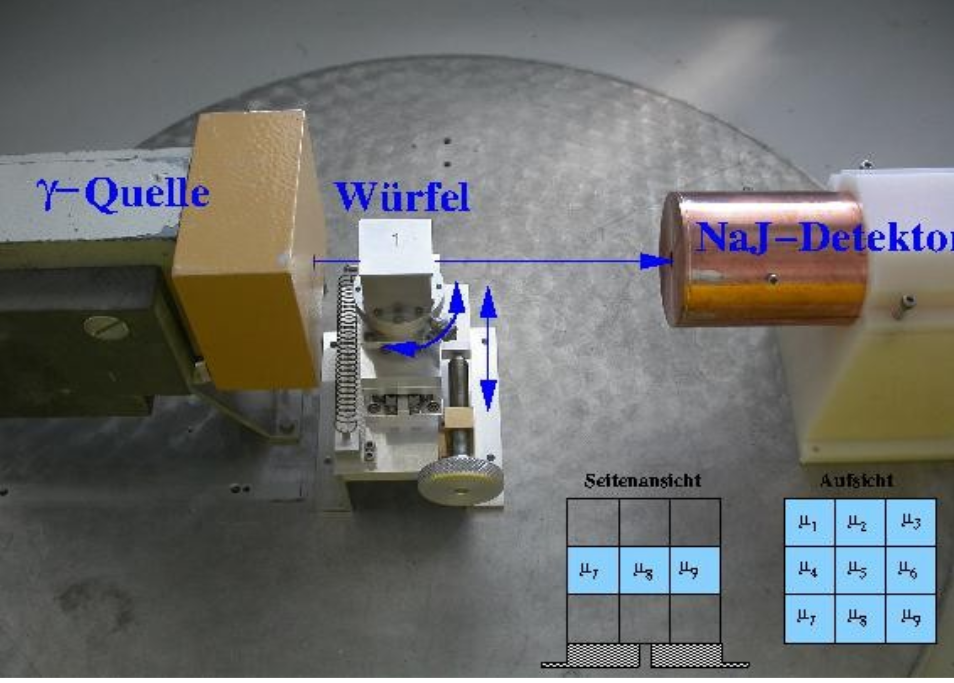
\includegraphics[height=6cm]{Aufbau.PNG}
  \caption{Grundlegender Aufbau des Versuchs. \cite{sample}}
  \label{fig:aufbau}
\end{figure}

Von einer Caesium-137-Quelle wird $\gamma$-Strahlung emittiert, welche durch eine
davor befindliche Blende kollimiert wird. Dahinter befindet sich dann eine rotierbare
Halterung, auf welcher verschiedene Würfel befestigt werden können.

Zur eigentlichen Messung der Zählraten dient ein NaJ-Detektor.
Dabei handelt es sich um einen sogenannten Szintillationsdetektor.
Beim Durchlaufen eines Szintillators, regen die Photonen der $\gamma$-Strahlung dessen
Moleküle durch Stoßprozesse an. Die Anregungsenergie wird anschließend wieder in Form
von Licht abgegeben. Hierdurch entstehende Lichtimpulse sind sehr schwach und
werden daher mithilfe eines Photomultipliers verstärkt. Die Photonen treffen dabei
auf eine Photokathode, wodurch Elektronen aus dieser ausgelöst werden (Photoeffekt).
Diese Elektronen werden dann in einem elektrischen Feld beschleunigt und treffen
schließlich auf weitere Elektroden. Da sie aufgrund der Beschleunigung Energie
aufgenommen haben, sind sie ihrerseits in der Lage mehrere
Elektronen aus den Elektroden auszulösen. Dadurch wird die Anzahl der Elektronen lawinenartig erhöht
und es kann letztendlich ein Stromimpuls gemessen werden, dessen Amplitude von der
Energie der einfallenden Strahlung abhängig ist. Die Messung geschieht über einen Vielkanalanalysator.

Der Vielkanalanalysator "sortiert" dabei praktisch die gemessenen Stromimpulse nach ihrer Höhe.
Dies geschieht im Wesentlichen durch einen Analog-Digital-Converter und einen Datenspeicher mit bestimmt vielen
Speicherplätzen (Kanälen). Der ADC wird beim Eintreffen eines Impulses aktiv und bestimmt eine ganze Zahl, welche
dem der Impulsamplitude proportionalen Wert am nächsten kommt (dazu muss vorher ein Proportionalitätsfaktor eingestellt
werden). An dem der Zahl entsprechenden Speicherplatz wird zum dort vorhandenen Wert eine Eins addiert. Dadurch
kann am Ende der Messung dann überprüft werden, wie viele Impulse es mit Amplituden in einem bestimmten Bereich gegeben hat.

Die Ergebnisse der jeweiligen Messung werden über einen am Detektor angeschlossenen PC ausgegeben.

Insgesamt werden die Zählraten bei einer Abschwächung durch 4 verschiedene Würfel gemessen.
Bei Würfel 1 und 4 werden die Zählraten für 12 verschiedene Anordnungen der Würfel bestimmt.
Bei Würfel 2 und 3 lediglich für 4 Anordnungen. Lediglich bei Würfel 1 werden die Zählraten über einen
Zeitraum von $\SI{100}{\second}$ gemessen. Bei den anderen Würfeln jeweils über einen
Zeitraum von $\SI{300}{\second}$.
